\documentclass[12pt,openright,twoside,a4paper,brazil,english]{abntex2}
\usepackage{lmodern}
\usepackage[T1]{fontenc}
\usepackage[utf8]{inputenc}
\usepackage{lastpage}
\usepackage{indentfirst}
\usepackage{color}
\usepackage{graphicx,graphicx}
\usepackage{epsfig,subfig}
\usepackage{microtype}
\usepackage{lipsum}	
\usepackage{amsmath,amssymb,mathrsfs}
\usepackage{setspace}
\usepackage{verbatim}
\usepackage{tabularx}
\usepackage{afterpage}
\usepackage{url} 
\usepackage[brazilian,hyperpageref]{backref}
\usepackage[alf]{abntex2cite}
% --- 
% CONFIGURAÇÕES DE PACOTES
% --- 

% ---
% Configurações do pacote backref
% Usado sem a opção hyperpageref de backref
\renewcommand{\backrefpagesname}{Citado na(s) página(s):~}
% Texto padrão antes do número das páginas
\renewcommand{\backref}{}
% Define os textos da citação
\renewcommand*{\backrefalt}[4]{
	\ifcase #1 %
		Nenhuma citação no texto.%
	\or
		Citado na página #2.%
	\else
		Citado #1 vezes nas páginas #2.%
	\fi}%
% ---
\titulo {Análise de Discrepância da Bibliografia do Mahdi E Proposta de Modelo CubeSats Didático}
\autor{Gabriel Alves Silva}
\local{Santo André - SP}
\data{22 de fevereiro de 2022}
\orientador{Antonio Gil Vicente de Brum}
\coorientador{}
\instituicao{Universidade Federal do ABC
  \par
  Centro de Engenharia, Modelagem e Ciências Sociais Aplicadas 
  \par
  Programa Graduação em Engenharia Aeroespacial}
\tipotrabalho{Trabalho de Graduação (Engenharia Aeroespacial)}
\preambulo{\textbf{Trabalho de Graduação} apresentada ao Programa de Graduação em Engenharia Aeroespacial, como parte dos requisitos necessários para a obtenção do Título de Bacharel em Engenharia Aeroespacial.}
% ---
%  Configurações de aparência do PDF final
% NÃO ALTERAR!!!

% alterando o aspecto da cor azul
\definecolor{blue}{RGB}{41,5,195}

% informações do PDF
\makeatletter
\hypersetup{
     	%pagebackref=true,
		pdftitle={\@title}, 
		pdfauthor={\@author},
    		pdfsubject={\imprimirpreambulo},
	    pdfcreator={LaTeX with abnTeX2},
		pdfkeywords={abnt}{latex}{abntex}{abntex2}{trabalho acadêmico}, 
		colorlinks=true,       		% false: boxed links; true: colored links
    		linkcolor=blue,          	% color of internal links
    		citecolor=blue,        		% color of links to bibliography
    		filecolor=magenta,      		% color of file links
		urlcolor=blue,
		bookmarksdepth=4
} 
\makeatother
% --- 
\setlength{\parindent}{1.3cm}
\setlength{\parskip}{0.2cm}
\makeindex
\begin{document}
\frenchspacing
\pretextual
\begin{capa}
\centering
\LARGE{Universidade Federal do ABC\\}
\large{Centro de Engenharia, Modelagem e Ciências Sociais Aplicadas}
    \vfill
    \begin{figure}[h!]
        \centering
        
\includegraphics[scale=1.2]{figs/logo.png}
    \end{figure}
    \vfill
    \Large\imprimirautor
	\vfill
\textbf{\LARGE\imprimirtitulo}
	\vfill
    \Large\imprimirorientadorRotulo~\imprimirorientador\\
    \Large\imprimircoorientadorRotulo~\imprimircoorientador
    
    \vfill
    \vfill
    \large\imprimirdata\\
    \large\imprimirlocal
\end{capa}


\imprimirfolhaderosto*

% ---
% Ficha Catalográfica
% ---
% Isto é um exemplo de Ficha Catalográfica, ou ``Dados internacionais de
% catalogação-na-publicação''. Você pode utilizar este modelo como referência. 
% Porém, talvez a biblioteca lhe fornece um PDF
% com a ficha catalográfica definitiva após a defesa do trabalho. Quando estiver
% com o documento, salve-o como PDF no diretório do seu projeto e substitua todo
% o conteúdo de implementação deste arquivo pelo comando abaixo:
%
% \begin{fichacatalografica}
%     \includepdf{fig_ficha_catalografica.pdf}
% \end{fichacatalografica}
\begin{fichacatalografica}
	\vspace*{\fill}					% Posição vertical
	\hrule							% Linha horizontal
	\begin{center}					% Minipage Centralizado
	\begin{minipage}[c]{12.5cm}		% Largura
	
	\imprimirautor
	
	\hspace{0.5cm} \imprimirtitulo  / \imprimirautor. --
	\imprimirlocal, \imprimirdata-
	
	\hspace{0.5cm} \pageref{LastPage} p. : il. (algumas color.) ; 30 cm.\\
	
	\hspace{0.5cm} \imprimirorientadorRotulo~\imprimirorientador\\
	
	\hspace{0.5cm}
	\parbox[t]{\textwidth}{\imprimirtipotrabalho~--~\imprimirinstituicao,
	\imprimirdata.}\\
	
	\hspace{0.5cm}
		1. Palavra-chave1.
		2. Palavra-chave2.
		I. Orientador.
		II. Universidade xxx.
		III. Faculdade de xxx.
		IV. Título\\ 			
	
	\hspace{8.75cm} CDU 02:141:005.7\\
	
	\end{minipage}
	\end{center}
	\hrule
\end{fichacatalografica}
% ---
% ---
% Assinaturas
% ---
% Isto é um exemplo de Folha de aprovação, elemento obrigatório da NBR
% 14724/2011 (seção 4.2.1.3). Você pode utilizar este modelo até a aprovação
% do trabalho. Após isso, substitua todo o conteúdo deste arquivo por uma
% imagem da página assinada pela banca com o comando abaixo:
%
% \includepdf{folhadeaprovacao_final.pdf}
%
\begin{folhadeaprovacao}

  \begin{center}
    {\large\imprimirautor}

    \vspace*{\fill}\vspace*{\fill}
    \begin{center}
      \textbf{\Large\imprimirtitulo}
    \end{center}
    \vspace*{\fill}
    
    \hspace{.45\textwidth}
    \begin{minipage}{.5\textwidth}
        \imprimirpreambulo
    \end{minipage}%
    \vspace*{\fill}
   \end{center}
        
 % Isso na versao final do trabalho!!!       
   Trabalho aprovado. \imprimirlocal, 01 de janeiro de 2014:

   \assinatura{\textbf{\imprimirorientador} \\ Orientador} 
   \assinatura{\textbf{\imprimircoorientador} \\ Co-Orientador} 
   \assinatura{\textbf{Professor} \\ Convidado 1}
   \assinatura{\textbf{Professor} \\ Convidado 2}
   \assinatura{\textbf{Professor} \\ Convidado 3}
      
   \begin{center}
    \vspace*{0.5cm}
    {\large\imprimirlocal}
    \par
    {\large\imprimirdata}
    \vspace*{1cm}
  \end{center}
  
\end{folhadeaprovacao}
% ---
% ---
% Dedicatória
% ---
\begin{dedicatoria}
   \vspace*{\fill}
   \centering
   \noindent
   \textit{ Aos verme que roeu as frias carnes de meu cadáver.} \vspace*{\fill}
\end{dedicatoria}
% ---
% ---
% Agradecimentos
% ---
\begin{agradecimentos}



Agradeço a Xuxa, meus pais, cachorro, gato e papagaio, por ...

Agradeço ao meu orientador, XXXXXXXXX, por todos os conselhos, pela paciência e ajuda nesse período.

Aos meus amigos ...

Aos professores ...

À XXXXXX pelo apoio financeiro para realização deste trabalho de pesquisa.

\end{agradecimentos}
%% ---
% ---
% Epígrafe
% ---
\begin{epigrafe}
    \vspace*{\fill}
	\begin{flushright}
		\textit{``Não sei o que, \\
		          não sei o que,\\
                  não sei o que lá.''\\
		          (Autor Desconhecido)}
	\end{flushright}
\end{epigrafe}
% ---
% ---
% RESUMOS
% ---

% RESUMO em português
\setlength{\absparsep}{18pt} % ajusta o espaçamento dos parágrafos do resumo
\begin{resumo}
A atitude de um veículo refere-se à orientação dos eixos de coordenadas fixos no corpo em relação a um referencial definido e o controle de atitude, por sua vez, são as técnicas para manter a orientação do corpo dentro dos limites definidos. Dentro das técnicas conhecidas, têm-se a modelagem Newton-Kepler para dinâmica orbital, a de Newton-Euler para rotação de corpos rígidos e o controle proporcional inercial derivativo para o controle de atitude. O presente trabalho de graduação com o objetivo de atestar o aprendizado apresenta o estudo, modelagem e análise da mecânica orbital e rotacional abordando o controle de atitude de um CubeSat em órbita circular. Ao decorrer do trabalho será feita comparação com a literatura e apontamento de discrepâncias e proposta de abordagem.

 \textbf{Palavras-chaves}: CubeSat, Controle de Satélites, Dinâmica e Controle de Veículos Espaciais, Controle PID, Dinâmica Orbital.
\end{resumo}

% ABSTRACT in english
\begin{resumo}[Abstract]
 \begin{otherlanguage*}{english}
   This is the english abstract.

   \vspace{\onelineskip}
 
   \noindent 
   \textbf{Keywords}: latex. abntex. text editoration.
 \end{otherlanguage*}
\end{resumo}
% Lista de ilustrações
\pdfbookmark[0]{\listfigurename}{lof}
\listoffigures*
\cleardoublepage

% Lista de tabelas
\pdfbookmark[0]{\listtablename}{lot}
\listoftables*
\cleardoublepage

% Lista de abreviaturas e siglas
\begin{siglas}
  \item[ABNT] Associação Brasileira de Normas Técnicas
  \item[abnTeX] Normas para TeX
\end{siglas}

% Lista de símbolos
\begin{simbolos}
  \item[$ \Gamma $] Letra grega Gama
  \item[$ \Lambda $] Lambda
  \item[$ \zeta $] Letra grega minúscula zeta
  \item[$ \in $] Pertence
\end{simbolos}

% Inserir o SUMÁRIO
\pdfbookmark[0]{\contentsname}{toc}
\tableofcontents*
\cleardoublepage
\textual
\pagenumbering{arabic}
\setcounter{page}{1}
\chapter*[Introdução]{Introdução}
\addcontentsline{toc}{chapter}{Introdução}

O acúmulo do avanço técnico-científico até o final do século XIX permitiu que a humanidade  superasse o caráter de espectador para protagonista na exploração do espaço. Quando adentrado o século XX essa exploração evolui, se tornando fundamental para a evolução da sociedade e soberania das nações. Foi naquele século que as técnicas foram desenvolvidas para acompanhamento e estruturação das missões, tripuladas ou não, que alcançaram e estudaram nossa vizinhança. Do cenário belicoso da Guerra Fria frutifica os programas Sputnik, Explorer, Vostok, Gemini, Apollo etc, que caracterizam, uma “era de ouro”, a corrida espacial compreendida entre 1953 a 1975.

Com  o final da Guerra Fria se inaugura uma cultura de cooperação entre as diversas agências espaciais do mundo, e adiciona a participação cada vez mais presente do setor privado. E é nesse novo contexto que surge uma nova corrida espacial, com várias faces: exploração de recursos espaciais, presença de longo prazo em estações e corpos celestes e exploração de Marte. Na transição dos séculos já são fundados dois grandes nomes do setor privado espacial, a Blue Origin (2000) e a SpaceX (2002). E em menos 15 anos, em 2016, Elon Musk fundador, CEO e CTO da SpaceX estava apresentando no 67º Congresso Internacional Astronáutico “Interational Astronautical Congress (IAC)”, Guadalajara - México, o plano “Mars and Beyond” com o ano de 2023 para começar os voos tripulados para Marte em seu cronograma. Em 2017 o Presidente dos Estados Unidos, Donald Trump, assina uma nova política espacial nacional, que prevê o trabalho em conjunto da Nasa com setores privados, com o objetivo de retornar à Lua e explorar Marte, programa batizado em 2019 de Artemis.

1972 a Apollo 17 foi a última missão tripulada à Lua, após, a presença humana no espaço teve como limite a órbita terrestre baixa, protegida pelo campo magnético da Terra. O espaço externo ao escudo de proteção magnético que a Terra oferece, é danoso tanto para equipamentos eletrônicos quanto para organismos vivos. De onde emergem os desafios para a exploração de Marte, assentamento na Lua e mineração de corpos celestes, tais desafios fomentam a seguinte estratégia: estudo do ambiente espacial por missões não tripuladas de baixo custo.

Os CubeSats por suas características de: modularidade, uso de componentes de prateleira menor custo e difusão nas diversas agências espaciais, institutos de pesquisa e educação ao redor do mundo. O torna a solução imediata lógica para missões além da órbita baixa terrestre com o objetivo de estudar o ambiente espacial, testar componentes, testar técnicas e métodos e mapear asteroides, a Lua e Marte. Assim, para a demonstração de tecnologia, foram desenvolvidas os CubeSats gêmeos de comunicação MarCo A e B, com o objetivo de demonstrar a capacidade de comunicação com a sonda terrestre Insight e a Terra.  Outro exemplo é a missão Artemis I, na qual a NASA ofereceu carregar treze CubeSats 6U para missões lunares e exploração do espaço profundo.

Desde 2014, têm-se participações do Brasil no estudo e uso de CubeSats, com a demonstração da capacidade e custos da plataforma, conclui-se ser cada vez mais adequada e preferível solução para a exploração dos recursos espaciais. Em conjunto, a Agência Espacial Brasileira, os Institutos de Pesquisa e a Universidade trabalham em conjunto para dominar tal plataforma. Temos como exemplo o Nanosatc-Br, ItaSat, Serpens. E mais recentemente o Pion-BR1, primeiro satélite criado por um startup brasileira, lançado pelo foguete Falcon 9, da SpaceX.

Para auxiliar a entrada do Brasil no estudo do espaço além das órbitas baixas terrestres e acompanhar as tendências apresentadas acima, o objeto de estudo deste trabalho de conclusão de curso está inserido na grande área de Dinâmica e Controle da Engenharia Aeroespacial. Sendo ele o estudo da resposta PID de um CubeSat em uma órbita circular.

O presente estudo é dividido em seis capítulos, apresentados a seguir:

O Capítulo 1 apresenta referências utilizadas.

O capítulo 2 inicia sobre as ferramentas, técnicas e plataformas exploradoras e o grau de inovação das mesmas.  

O capítulo 3 aprofunda os conceitos relacionados ao desenvolvimento do presente estudo, os fundamentos físicos para a modelagem, as estratégias para o controle do modelo e as referências para os atuadores.

O capítulo 4 desenvolve a metodologia para a aquisição dos dados que permitem a comparação, além das ferramentas utilizadas.

O capítulo 5 apresenta de forma clara, o que está sendo proposto no estudo, métricas usadas e considerações no processo.

O capítulo 6 apresenta os resultados obtidos na simulação e discussão do mesmo.

O capítulo 7 e final, é a conclusão do projeto.
\section*{Motivação:}\label{sec:Motivação:}
\addcontentsline{toc}{section}{Motivação:}
No contexto de aluno de graduação, o presente trabalho de conclusão de curso da engenharia aeroespacial, busca auxiliar os pares do autor, com a apresentação do conteúdo referente de forma sintética, didática e centralizada. Para exploração do tema, tanto em iniciações científicas ou competições acadêmicas relacionadas.
\section*{Objetivo:}\label{sec:Objetivo:}
\addcontentsline{toc}{section}{Objetivo:}
Este trabalho tem como objetivo a síntese e aplicabilidade direta dos conhecimentos adquiridos no curso de Engenharia Aeroespacial da Universidade Federal do ABC.

O tema do estudo é dinâmica orbital e rotacional e controle PID de CubeSats. O foco neste estudo é explorar a literatura e a partir da modelagem computacional visualizar o comportamento da trajerória e atitude e a respota do controlador PID. Para isso usou-se as ferramentas de MATLAB e SIMULINK e por fim Octave na reprodução e análise de livros e trabalhos académicos.
\subsection*{Objetivo Geral:}
\begin{itemize}
\item  Reproduzir de forma computacional a mecânica rotacional e orbital de um CubeSat e da resposta do controlador PID. 
\end{itemize}

\subsection*{Objetivo Expecífico:}
\begin{itemize}
\item Modelar mecânica orbital de um CubeSat.
\item Apresentar visão 3D e tracejado de Solo da Órbita.
\item Modelar mecânica orbital de um CubeSat.
\item Apresentar gráficos do comportamento rotacional não controlado.
\item Modelar sistema de Controle PID para um CubeSat.
\item Afinação do controlador PID pelo método de Ziegler Nichols.
\item Analisar resposta encontrada pelo controlador.
\end{itemize}


\part{Preparação da pesquisa}
\chapter{Revisão Literária}

Esse capítulo está dedicado em apresentar e comentar brevemente a literatura empregada no desenvolvimento deste trabalho. São divididas em três tipos, de acordo com sua utilidade:

\section{Obras de exploração temática:}

Mediante a amplitude dos temas abordados na engenharia aeroespacial e ainda da área de Dinâmica e Controle, as seguintes obras são de onde o estudo prospectou a problemática e o tema a ser analisado:

Do periódico IEEE-AESM de volume 35 número 3, referente ao mês de março de 2020. Foi uma edição especial com editores convidados do JPL, do Centro Espacial de Surrey da Universidade de Surrey e da Universidade do estado da Califórnia. Para apresentar o potencial dos CubeSats que a Nasa ofereceu lançar  como carga paga da missão teste do Artemis I. Nesta edição destaca os planos de diversas universidades e centros de pesquisa ao redor do mundo em usar os CubeSat em diversos tipos de missão, incluindo, exploração de asteroides, mapeamento e estudo do espaço profundo. O que auxiliou no desenvolvimento da problemática aqui trabalhada.

Das apresentações dos planos Artemis revisão 2020 e Plano Mars and Beyond revisão 2022. Atualmente os dois nomes mais famosos na exploração espacial, desses documentos, retira-se as tendências e sub tendências para o mercado aeroespacial do mundo.

 O Resumo Executivo CubeSats, CGEE, 2018, oferece uma apresentação clara sobre de onde vieram os CubeSats, quais foram seus propósitos na época e atualmente, definições técnicas entre outras informações necessárias para o real entendimento dessa plataforma tecnológica.
 
Das colunas: NASA Space Launch System’s First Flight to Send Small Sci-Tech Satellites Into Space - fevereiro de 2016; JPL  MarCo - revisão 2022; IEEE Spectrum Nasa’s Space Launch System will lift off, but with rival rockets readying for flight, the value of SLS is murky; Canaltech: Satélite criado por startup brasileira será lançado pela SpaceX em 2022 - dezembro de 2021. Oferecem uma perspectiva temporal dos acontecimentos envolvendo os tópicos encontrados nas leituras supracitadas, uma noção de atualidade que acaba se perdendo nos periódicos.

Na apresentação: O Desenvolvimento de CubeSats no Brasil - INPE - SeCiAer 2018, Apresentada no seminário de serviços científicos e aeronáuticos de 2018, oferece de forma visual e resumida as iniciativas dos diversos atores brasileiros na exploração espacial com o uso da plataforma CubeSats, incluindo dados como Nome, anos, missão e um resumo e resultado dessas iniciativas.

Explorando os endereços eletrônicos oficiais das empresas PION-Labs, Nanoavionics, Blue Canyon, é prospectado informações relevantes   das plataformas, dispositivos e missões que essas plataformas serão utilizadas, esclarecendo assim a posição que startups e pequenas empresas ocupam nesse mercado.

\section{Obras do estado da arte:}

O entendimento do estado da arte é apresentado a seguir na seara do Estado da Arte, onde serão explorados os assuntos relacionados e estado atual de tais assuntos. Foi usado de referência:

CubeSat 101: Basic Concepts and Processes for First-Time CubeSat Developers, outubro de 2017, que explica de forma mais técnica como é feito um CubeSat, tamanhos e parâmetros a se atentar. Leitura fundamental e primária para entender a plataforma tecnológica.

Dos artigos e trabalhos académicos Development of models for Attitude Determination and Control System components for CubeSat applications; Sistema de Controle de Atitude Proposto para a Missão Espacial SERPENS II. Análise Comparativa de Técnicas de Controle de Atitude Aplicadas à Simulação de uma Planta Baseada nos Satélites do Tipo CubeSat. Foram as bases para a reprodução e aplicação do conhecimento adquirido pelo estudo do referencial teórico.

\section{Obras para referencial teórico:}

Os aspectos teóricos das seguintes referências, são aprofundados na Fundamentação Teórica. Ademais segue uma explicação de como cada capítulos e seções são estruturados e utilizados nessa fundamentação, trazendo algumas considerações.

O livro, Attitude Stabilization for CubeSats - Mohammed Chessab Mahdi, é a espinha do presente estudo. Como expõe de forma didática e centralizada informações especializadas para a plataforma de CubeSats se alinha com as motivações e objetivos para o trabalho. O capítulo 3 é usado  na modelagem da dinâmica de atitude do satélite, o capítulo 4 refere-se ao sistema de controle, assim as seções 4.1 a 4.3 que se referem ao controle proporcional integral e derivativo fundamentam o modelo de controle aqui desenvolvido finalmente o capítulo 5 que se trata da simulação desse sistema de controle e modelo em MATLAB e SIMULINK nas seções 5.1 e 5.2 se mostram úteis para a obtenção e análise de dados.

Vale a seguinte consideração sobre a referência citada imediatamente acima: Ao longo do estudo o autor do atual trabalho mesmo aplicando cuidadosamente as técnicas e formulações apresentadas no livro, não alcançou de forma confiável os resultados apresentados. Separando assim, uma subsecção na metodologia, para exploração do acontecido.  

Mediante à incerteza da consideração acima, por precaução e redundância foi utilizado o livro Space Vehicle Dynamics and Control, Bong Wie, aferir e complementar o desenvolvimento teórico do livro anterior. O Capítulo 2 das seções 2.1 a 2.3 conferem o sistema de controle dinâmico. O capítulo 3 das seções 3.4 a 3.7 conferem o modelo dinâmico referente a órbita do suposto satélite, tal modelo é utilizado nas seções seguintes, o capítulo 5 é completamente usado para o entendimento do equacionamento da dinâmica rotacional usado a seguir no capítulo 6 do qual foi retirado das seções 6.1 a 6.11 a validação do modelo dinâmico do satélite, por fim o capítulo 7 da seção  7.1 a 7.2 vem os equacionamentos para o sistema de controle, tanto magnético quando por rodas de momento.

Acompanhando esses modelos dinâmicos, para a modelagem mais fidedigna da roda de reação e torqueadores magnéticos é usado o clássico, Spacecraft Attitude Determination and Control editado pelo Wetz, tópicos referenciados nos capítulos 6 seção 6.6 e 6.7 e juntamente o  capítulo  7 seções 7.5 e 7.9.

Para o desenvolvimento do sistema de controle proporcional, integral e derivativo, é usado o livro Engenharia de Controle Moderno, do  Ogata, o capítulo 8 que se referente ao projeto de controladores PID.

\chapter{Estado da Arte}\label{cap:Estadp da Arte}
\section{CubeSats}\label{sec:CubeSats}
CubeSat são nanosatélites com normas rígidas de padronização. Desenvolvidos pela colaboração entre Puig-Suari, professor da Universidade Estadual Politécnica da Califórnia e Bob Twiggs, professor da Universidade de Stanford, com o intuito de acessibilizar o espaço. Essa plataforma apesar de apresentar uma variedade de tamanhos, todas se baseiam na unidade padrão de CubeSat, mais conhecida como 1U.

Uma unidade padrão de CubeSat, 1U, refere-se a um cubo de 10cm de arestas e a massa entre 1kg e 1.33kg. As demais configurações se devem à união ou adaptação dessa unidade. Por exemplo, um CubeSat 2U tem dimensões de massa de dois 1U conectados, 3U segue a mesma lógica só que três unidades 1U conectadas longitudinalmente. Essas configurações devem levar em consideração qual será o Sistema Dispensador de CubeSats, CubeSat Dispenser Systems.

O Sistema Distribuidor de CubeSats é a interface que conecta o CubeSat com o veículo lançador. Suas principais funções são fixação no veículo lançador, proteção do CubeSat durante o lançamento e liberação do mesmo no espaço no momento apropriado. Os mais comuns são o Dispensador 3U, e depois do sucesso da plataforma foi concebido em 2014, o Dispensador 6U, no referente tempo em que esse trabalho foi escrito tem-se Dispensadores para configurações ainda maiores.

O Biosentinel é um CubeSat 6U que estuda o comportamento de compostos orgânicos no espaço.  O Equuleus outro 6U estuda o ponto lagrangeano Terra-Lua L2 e testa um sistema de propulsão por jatos de água combinado com um sistema de determinação e controle de atitude de prateleira da Blue Canyon. O Serperns II com configuração 3U, é uma plataforma de capacitação de alunos e profissionais da área.

A NanoAvionics é um exemplo de empreendedorismo privado na área de nano e micro satélites. Começando sua história com um cubesat 1U e desenvolvendo tecnologia, acúmulo de conhecimento e crescimento iterativo. Foram desenvolvidos satélites multiuso: M3P, M6P, M12P e M16P e paulatinamente demonstrando o domínio da tecnologia dos padrões CubeSat 3U, 6U, 12U e 16U. Atualmente  oferece a plataforma comercial  do microssatélite MP42 modular (até 115kg).

Realizou em 2015, junto com o Centro Nacional de Ciências Físicas e Tecnologia da Lituânia, um projeto de materiais catalíticos para sistemas de propulsão monopropelente miniaturizados. Em 2018 esta empresa especializada em soluções para missões de satélites, sendo elas de propósito comercial ou científica, teve AST 'I\&' Science adquirindo o  seu controle acionário e recebendo em 2019 a bolsa Horizon 2020 da UE e da ESAA.

O modelo de negócio da Nanoavionics vem sendo protagonizado no Brasil pela PION, primeira empresa privada brasileira a lançar um CubeSat. Atualmente eles dominam a tecnologia 1U e comercializam modelos educacionais.

O desenvolvimento de um CubeSat depende completamente da missão na qual vai empenhar. Focando no documento base do assunto “CubeSat 101 Basic Concepts and Processes for First-Time CubeSat Developers” um CubeSat pode levar da fase conceitual até ser entregue para o lançamento de nove a vinte e quatro meses. Sua missão irá definir  os requisitos de órbita, lançadores, e componentes.

 De todas as missões da Iniciativa de Lançamento de CubeSat (Nasa CSLI), metade conduzem missões científicas, sessenta e seis por cento conduzem demonstrações de tecnologia. Como exemplo temos: testes biológicos no espaço, estudo de objetos próximos da Terra NEO, comunicação entre CubeSats, navegação e controle, teste de radiação e ambiente espacial, entre outros. Cada missão terá parâmetros diferentes para os subsistemas do veículo espacial.
 
Para o desempenho adequado do Sistema de Determinação e Controle de Atitude é necessário a escolha correta de sensores, atuadores de algoritmos controladores. Existe no mercado uma ampla gama de sensores, atuadores e até ADCS completamente integrados, também existe a possibilidade da produção interna desses componentes para redução de custos.

 Os torqueadores magnéticos usados no PION-BR1 e o SERPENS II, são os atuadores para o controle de atitude mais utilizados em CubeSats. Isso devido à possibilidade de produção interna, ao valor e tamanho relativamente menores. O que o torna mais favorável para missões simples e configurações menores. Esses torqueadores são pouco precisos (5 a 10 graus de precisão de apontamento) e ficam inoperantes em ambientes de campo magnético tênue ou inexistente, como por exemplo ao passar pela região dos pólos.
 
 Para missões mais críticas, complexas, precisas e com configurações maiores. Podendo ser em volta da Terra ou até mesmo interplanetárias, os torqueadores magnéticos são substituídos por rodas de reação, essas são muito mais pesadas e aumentam consideravelmente o valor do CubeSat. São usadas por exemplo em CubeSats maiores como o 3U nanosatellite bus M3P, os 6U Equuleus e BioSentinel até mesmo o 16U nanosatellite bus M16P / M16P-R.
 
\section{O que é o sistema de determinação e controle de Atitude (ADCS)}\label{sec:O que é o sistema de determinação e controle de Atitude (ADCS)}

Para qualquer missão espacial, existe um estado desejado específico para a atitude do satélite. Para manter a operação do CubeSat dentro desse envelope de funcionamento, é utilizado dispositivos que medem essa diferença angular, a taxa de variação dessa diferença e acionam elementos que provocam momentos angulares corrigindo o estado para um desejado.

Existem no mercado diversos dispositivos que oferecem soluções para a determinação ou controle de atitude. Temos por exemplo o XACT-50 da Blue Canyon Technologies que é um sistema integrado que oferece solução completa de determinação de atitude, e controle por meio de rodas de reação.

Sendo essas duas supracitadas, determinação de atitude e controle de atitude duas faces diferentes do mesmo problema. Assim, além de soluções integradas, são vendidas soluções específicas, como sensores, atuadores, placas controladoras, entre outros.

\section{Estratégia magnética}\label{sec:Estratégia magnética}
Os torqueadores magnéticos são atuadores comuns para CubeSats, são fáceis de produzir e também há uma variedade grande no mercado.

Existem dois modelos principais, aqueles instalados em placas, e aqueles instalados nas extremidades ou em volta do CubeSat. Por exemplo, os vendidos pela CubeSat Shop: CubeTorquer and CubeCoil, ISIS Magnetorquer board, EXA MT01 Compact Magnetorquer, NCTR-M002 Magnetorquer Rod. 

Todos são fios de cobre enrolados em formato de bobinas, quando uma corrente elétrica passa por esses fios, um campo magnético é gerado e o que ger um momento magnético de controle.

\section{Estratégia de transferência de momento angular}\label{sec:Estratégia de transferência de momento angular}
Rodas de reação são dispositivos atuadores comuns para o controle de atitude de veículos espaciais em geral, essas  baseiam seu funcionamento na  transferência de momento angular, costumam ser arranjadas em três unidades para controlar a rotação nos três eixos.

 Por permitirem a correção de atitude com precisão, estes dispositivos têm operação mais complexa e são mais custosos. Apenas missões onde os requisitos do apontamento são mais sensíveis, costumam se utilizar esses atuadores. Por isso, como mencionado anteriormente, elas são menos comuns em CubeSats.
 
 Contudo, com missões mais rebuscadas, envolvendo exploração interplanetária, esses dispositivos vêm se tornando mais comuns, até comercializados,  a SatBus 4RW0 é um conjunto de 4 rodas de reação desenvolvidas pela NanoAvionics para seus CubeSats (M3P ao M16P) que podem ser encomendadas, permitindo o apontamento preciso para missões de alto nível, CubeSat Shop oferece a CubeWhell modelos de roda de reação avulso, e tem-se também a Blue Canyon com sistemas completamentes integrados de ADTC com rodas de reação acopladas.

\chapter{Fundamentação Teorica}\label{cap:Fundamentação Teorica}

Esse trabalho é desenvolvido a partir  do estudo dos conceitos fundamentais de dinâmica e controle de veículos espaciais. Nas seções a seguir são apresentados os elementos teóricos para a fundamentação da modelagem física e matemática, da trajetória de um veículo espacial em uma órbita circular, da dinâmica de rotacional de um corpo rígido e do controle proporcional, integral e derivativo .

\section{Sistemas de Coordenadas e medida do tempo}

É de fundamental importância para qualquer estudo da mecânica a determinação objetiva dos sistemas de referência, sendo eles o de coordenadas e o de tempo. O parâmetro para essa escolha é a facilitação da formulação, visualização e análise.  

\subsection{Sistema de coordenadas geocêntrico-equatorial inercial }

Esse sistema quando assumido que não é rotacional e fixo no espaço é compreendido como inercial. A origem de seus eixos $X_{SCGI}$, $Y_{SCGI}$, $Z_{SCGI}$, se encontra fixo no centro de massa da Terra, ou seja geocêntrico.

O eixo $X_{SCGI}$ tem como sentido o equinócio vernal $\Upsilon$, o eixo $Z_{SCGI}$ aponta para a normal do plano equatorial terrestre, ou seja, para o polo Norte celeste e o eixo $Y_{SCGI}$ completa a base ortogonal dextrogiro. Mostrado na Figura~\ref{fig:log}, 

\begin{figure}[htpb]
   \center
   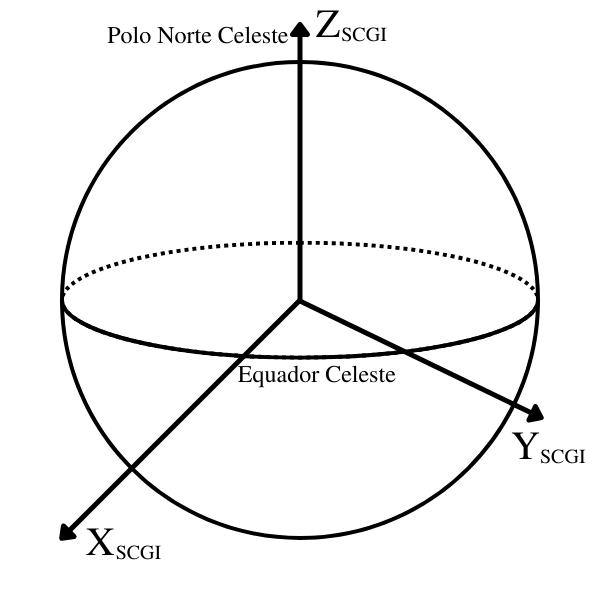
\includegraphics[scale=0.75]{figs/SCGI.PNG}
   \caption{Sistema de coordenadas geocêntrico-equatorial}
   \label{fig:log}
   \text{Fonte: Adaptada de "Fundamentals of Astrodynamics", Wertz, 1972}
\end{figure}

Esses eixos são determinados pela data de referência J2000 que é definido pela data Juliana referente ao dia 1º de Janeiro de 2000 as 12:00 tempo terrestre.

\subsection{Sistema de coordenadas orbital}

Esse sistema tem como origem o centro de massa do veículo espacial e seus eixos, $X_{SCO}$, $Y_{SCO}$, $Z_{SCO}$, acompanham sua órbita. O eixo $Z_{SCO}$ aponta em direção ao centro de massa da Terra ou, direção nominal do nadir. O eixo $Y_{SCO}$ tem como direção o oposto do vetor do plano de órbita do veiculo espacial. E o eixo $X_{SCO}$ aponta para o vetor velocidade ou, trajetória da órbita. Representado Figura~\ref{fig:log},

\subsection{Sistema de coordenadas fixo no corpo}

\section{Mecânica Orbital}
\subsection{Problema de dois corpos}
\subsection{Determinação dos elementos orbitais pelos vetores posição e velocidade}

\section{Dinâmica de Atitude}
\subsection{Matriz de cossenos diretores}
\subsection{Ângulos de Euler}
\subsection{Eixo-Angulo de Euler}
\subsection{Parâmetros de Euler - Quatérnions}
\subsection{Equações Diferenciais da Cinemática}
\subsection{Formulação Geral da Dinâmica de Corpo Rígido}
\subsection{Corpo Rígido em Órbita Circular}

\section{Determinação e Controle de Atitude}
\subsection{Algorítimo TRIAD}
\subsection{Filtro de Kalman}
\subsection{Técnica de Controle Proporcional Integral Derivativa}

\chapter{Materiais e Métodos}\label{cap:ferramentas}

\lipsum[12]
\section{Sistemas de Referência Orbita, Corpo e Inercial Equatorial Centrado na Terra}\label{sec:Sistemas de Referência}

O sistema de coordenadas geocêntrico-equatorial é escolhido como referencia inercial e global para o presente trabalho. Como o intervalo de estudo do fenômeno é irrelevante ao tempo de modificação desse sistema de referência tem-se como hipótese simplificadora que esse é considerado um sistema não rotativo, assumido como fixo no espaço.

\section{Fomulação de Newton-Kepler para Órbita}
\lipsum[12]

\section{Dinâmica Rotacional de Corpo Rígido de Newton-Euler}
\lipsum[12]

\section{Controle Proporcional, Integral, Derivativo}
\lipsum[12]

\section{Integração Numerica}
\lipsum[12]

\section{Octave}
\lipsum[12]

\section{Matlab}
\lipsum[12]

\section{Simulink}
\lipsum[12]

\part{Proposta}
\chapter{Sistema Proposto}\label{cap:proposta}

\lipsum[12]

\section{Posição, velocidade, elementos e trajetória orbitais}
\lipsum[12]
\subsection{Abordagem Analítica para Trajetória Orbital}
\lipsum[12]
\subsection{Abordagem Númerica para Trajétoria Orbital}
\lipsum[12]

\section{Reprodução da bibliografia "Attitude Stabilization for CubeSats: Concepts and Technology", Mahdi}
\lipsum[12]
\subsection{Capítulo 3: Modelagem da Dinâmica de Atitude de um Satélite}
\lipsum[12]
\subsection{Capítulo 5:Técnicas de Simulação do Controle de Atitude}
\lipsum[12]
\subsection{Discrepâncias}
\lipsum[12]

\section{Formulação didática de Modelo de atitude e controle de CubeSat}
\lipsum[12]
\subsection{Modelo da Dinâmica de Atitude de um Satélite}
\lipsum[12]
\subsection{Simulação de controle PID de Atitude}
\lipsum[12]
\subsection{Possíveis Formulações}
\lipsum[12]

\part{Parte Final}
\chapter{Resultados e Discussão}\label{cap:resultados}

\lipsum[73]

\section{Base de Dados}

\lipsum[72]

\section{Considerações Finais}

\lipsum[74]
\chapter*{Conclusões e Trabalhos Futuros}\label{cap:conclusao}
\addcontentsline{toc}{chapter}{Conclusão e Trabalhos Futuros}

\lipsum[81]

\section*{Conclusões}

\lipsum[82-84]

\section*{Trabalhos Futuros}

\lipsum[85] 
\postextual
\bibliography{bibliografia}
% ----------------------------------------------------------
% Apêndices
% ----------------------------------------------------------

% ---
% Inicia os apêndices
% ---
\begin{apendicesenv}

% Imprime uma página indicando o início dos apêndices
\partapendices
% ----------------------------------------------------------
\chapter{Primeiro Apêndice}
% ----------------------------------------------------------

\lipsum[50] % Texto qualquer. REMOVER!!

% ----------------------------------------------------------
\chapter{Segundo apêndice com título tão grande quanto se queira porque ele já faz a quebra de linha da coisa toda}
% ----------------------------------------------------------
\lipsum[51-53] % Texto qualquer. REMOVER!!

\end{apendicesenv}
% ---
% ----------------------------------------------------------
% Anexos
% ----------------------------------------------------------

% ---
% Inicia os anexos
% ---
\begin{anexosenv}

% Imprime uma página indicando o início dos anexos
\partanexos

% ---
\chapter{Nome do Primeiro Anexo}
% ---
\lipsum[30] % Texto qualquer. REMOVER!!

% ---
\chapter{Nome de Outro Anexo}
% ---

\lipsum[32] % Texto qualquer. REMOVER!!

\end{anexosenv}
\end{document}
